\apendice{Plan de Proyecto Software}

\section{Introducción}

La planificación de todo proyecto es un proceso de gestión organizado e integrado, centrado en las actividades necesarias para asegurar una exitosa consecución del proyecto. Esta planificación contribuye a una mejor utilización de los recursos, y a un uso óptimo del tiempo asignado a un proyecto, algo crucial en todo proyecto, y especialmente relevante en el caso de un Trabajo de Fin de Grado (TFG).

En este apartado se recogen los aspectos más relevantes en cuánto a la planificación temporal de nuestro proyecto, así como su viabilidad, tanto económica como legal.

\vspace{1cm}
\section{Planificación temporal}

Una de las primeras decisiones que se llevaron a cabo en el marco del proyecto JIZT, fue la elección de la metodología de desarrollo \emph{software} que adoptaríamos.

Lo primero que llevamos a cabo fue un análisis de las necesidades y limitaciones que presentaba nuestro proyecto, las cuales eran: tiempo limitado, eficiencia y velocidad, motivación y progreso del proyecto, y satisfacción de los usuarios.

Derivado de estas necesidades, se decidió que emplearíamos una metodología ágil. Las principales metodologías ágiles consideradas fueron Scrum, Kaban y Programación Extrema (XP).

Finalmente, nos decantamos por Kanban. Esta decisión estuvo en gran medida motivada por el hecho de que una planificación temporal rígida y prefijada, como ocurre por ejemplo en Scrum, era muy difícil de llevar a cabo en este proyecto dada nuestra inexperiencia con muchas de las herramientas y \emph{frameworks} utilizados.

Kanban nos permitía un flujo continuo de trabajo, permitiendo añadir historias de usuario no contempladas inicialmente si así se consideraba apropiado.

En total se estimaron 465 horas, de las cuales se emplearon realmente 464:

\begin{figure}[h]
	\centering
	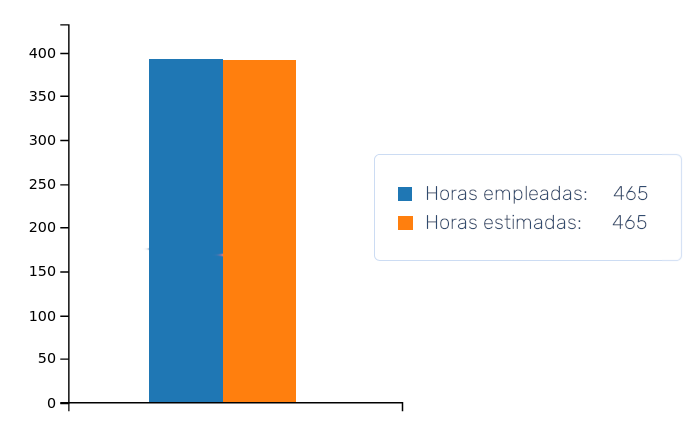
\includegraphics[width=0.6\textwidth]{hours-spent}
	\caption{Horas estimadas frente horas empleadas.}
\end{figure}

En esta planificación, se emplearon dos conceptos ágiles fundamentales:

\vspace{-0.3cm}
\begin{itemize}[\textbullet]
	\item \textbf{Historia de usuario}: se trata de una descripción de una funcionalidad del \emph{software} a implementar.
	\item \textbf{\emph{Epics}}: agrupan historias de usuario que conformen una misma \emph{feature}, o funcionalidad a desarrollar.
\end{itemize}

\vspace{-0.2cm}
En total, se especificaron 99 historias de usuario repartidas entre 8 \emph{epics}\footnote{Para la representación de las historias de usuarios y los \emph{epics} a GitHub se emplearon \emph{Issues} y \emph{Milestones}, respectivamente.}. Estos \emph{epics} fueron, ordenados de manera cronológica:

\vspace{-0.3cm}
\begin{itemize}[\textbullet]
	\item \textbf{Puesta en marcha}: tareas preliminares de organización y puesta en marcha del proyecto (elección de metodologías, herramientas, etc.).

	\item \textbf{Motor de Resumen v0.1}: implementar una primera versión del Motor de Resumen a través de los modelos preentrenados proporcionados por el módulo \texttt{transformers} de Hugging Face \cite{transformers}.

	\item \textbf{Arquitectura Microservicios v0.1}: implementar una primera versión reducida de la Arquitectura de Microservicios, configurando el componente Ingress de Kubernetes \cite{ingress}, y dos microservicios: el Dispatcher y el Pre-procesador de textos.
	
	\item \textbf{Arquitectura Microservicios v0.2}: continuar con la implementación de la arquitectura de microservicios, añadiendo la capacidad de realizar peticiones asíncronas y desarrollando la arquitectura dirigida por eventos. De momento, se sigue trabajando con una versión de la misma, esto es, con el Dispatcher y el  Pre-procesador de textos.

	\item \textbf{Arquitectura Microservicios v0.3}: una vez disponemos de una versión reducida de nuestra arquitectura que funciona correctamente en local, el siguiente paso es desplegarla en Google Kubernetes Engine (GKE) \cite{gke}. Además, se deben implementar los microservicios restantes (Codificador, Motor de Resumen y Post-procesador) y la base de datos para gestionar los resúmenes.
	
	\item \textbf{Cliente v0.1}: desarrollar el cliente (aplicación) que consumirá la API y permitirá al usuario final obtener resúmenes de sus textos. Dicho cliente se implementará con ayuda de Flutter \cite{flutter-es}, por lo que en principio estará disponible en plataformas móvil, \emph{web} y escritorio.
	
	\item \textbf{Arquitectura Microservicios v0.4}: ampliar la especificación de la API para que en las peticiones se puedan detallar todos los parámetros del resumen. Continuar con la mejora del sistema.
	
	\item \textbf{Documentación v0.1}: escribir la Memoria y los Anexos. Generar una primera versión de la documentación de la API REST y del código perteneciente a JIZT.
\end{itemize}

En la \autoref{gantt} se recoge un diagrama Gantt con el objetivo de facilitar la comprensión de la dimensión temporal del proyecto.

\begin{figure}[h]
	\centering
	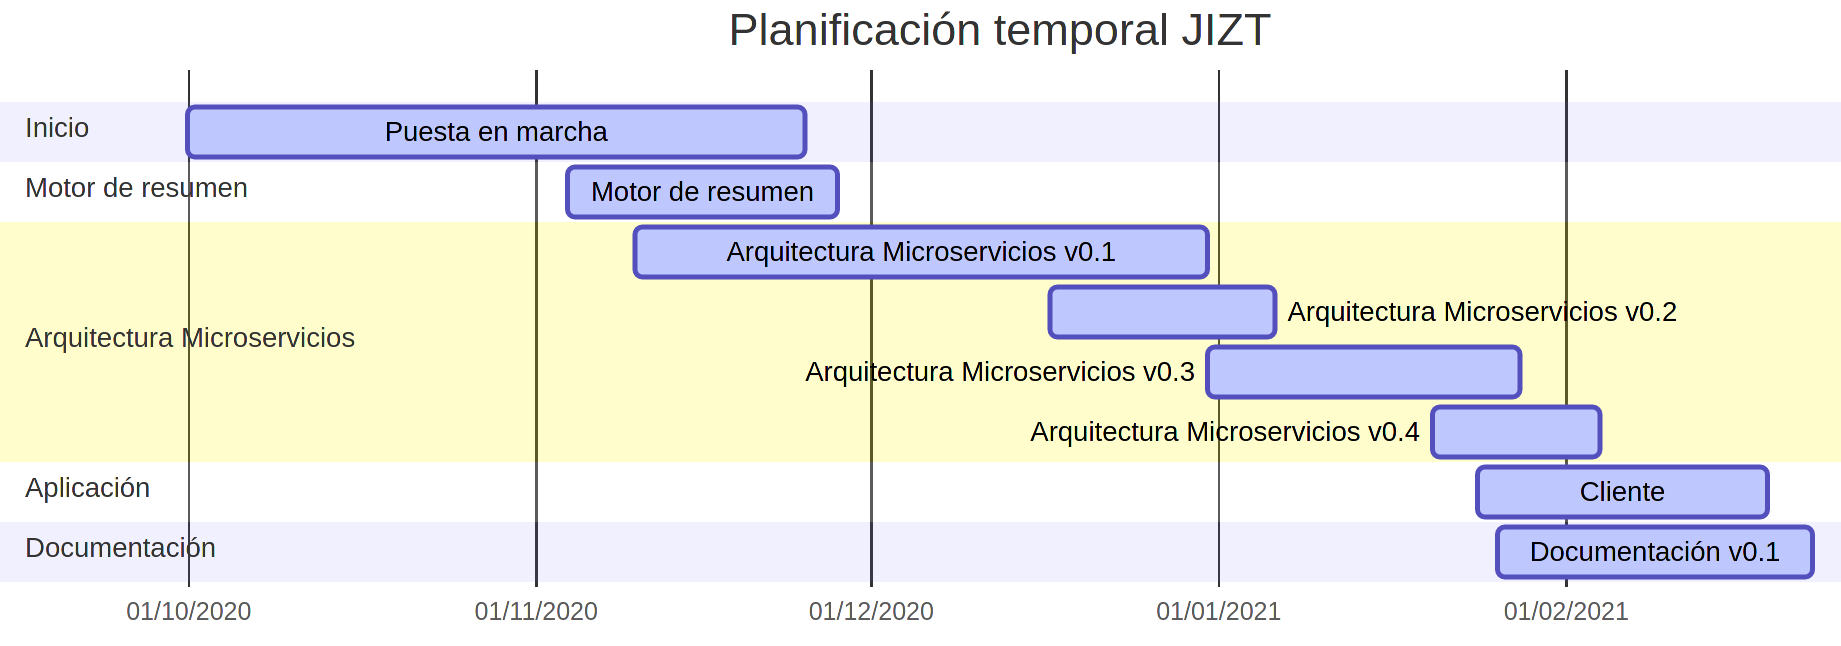
\includegraphics[width=\textwidth]{gantt-epics}
	\vspace{-0.6cm}
	\caption[Diagrama Gantt del proyecto.]{El proyecto comenzó el 1 de octubre de 2021, y finalizó el 16 de febrero de 2021.}
	\label{gantt}
\end{figure}

Dos conceptos importantes dentro de la metodología son \emph{lead time} y \emph{cycle time} \cite{anderson10}. Veamos qué significa cada uno de ellos.

\vspace{-0.3cm}
\begin{itemize}[\textbullet]
	\item \emph{Lead time}: es el período que transcurre entre la aparición de una nueva tarea en el flujo de trabajo y su salida final del sistema. Dicho de otro modo, es el tiempo total que el cliente está esperando la entrega de una parte del producto.
	
	\item \emph{Cycle time}: es la cantidad de tiempo que el equipo realmente empleó en una tarea, es decir, no se cuenta el tiempo que una tarea estuvo <<en espera>>. Por lo tanto, el tiempo del ciclo debe comenzar a medirse cuando la tarea pasa a la columna <<trabajando>>, y no antes.
\end{itemize}

\begin{figure}[h]
	\centering
	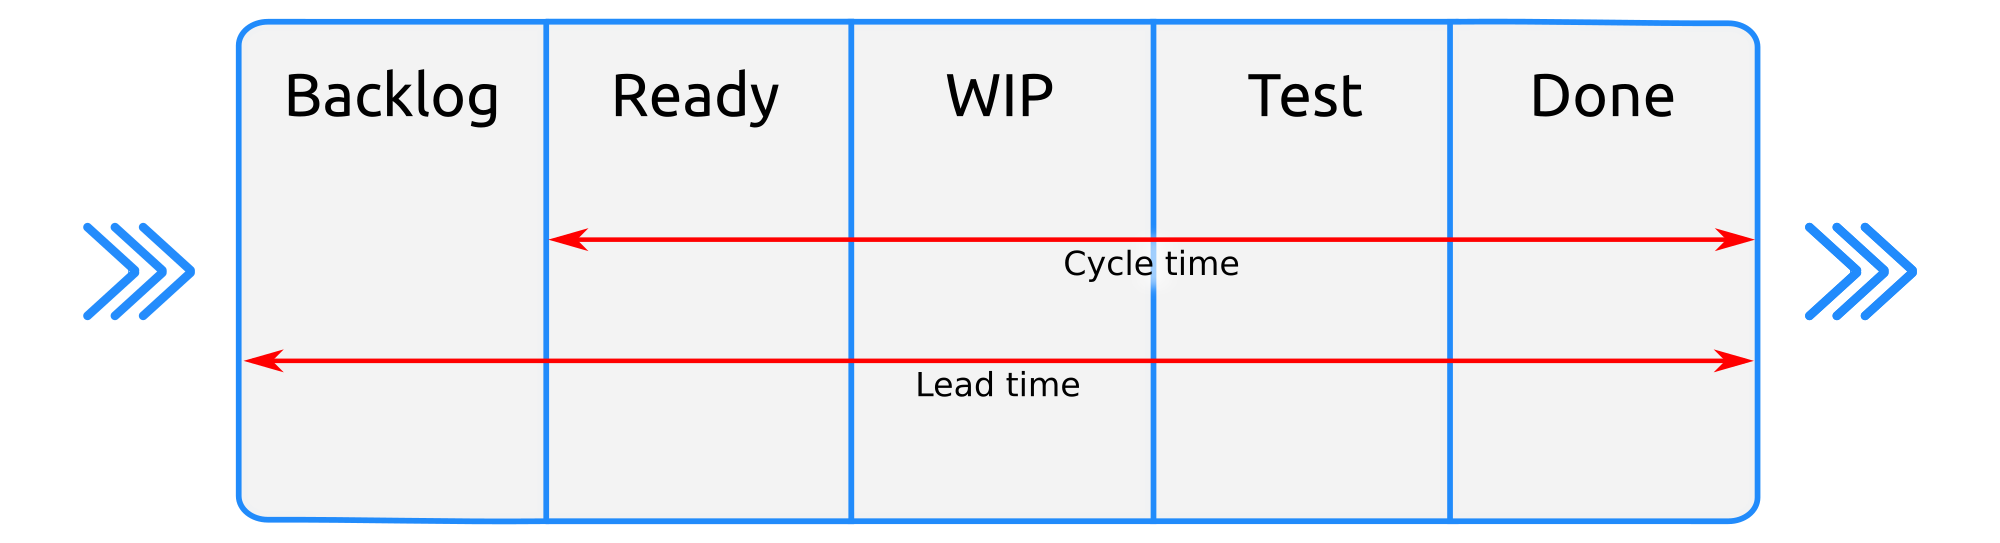
\includegraphics[width=\textwidth]{lead-cycle-time}
	\vspace{-0.6cm}
	\caption[Visualización del \emph{lead} y \emph{cycle time}.]{Explicación gráfica del \emph{lead} y \emph{cycle time} sobre un tablero Kanboard.}
\end{figure}

Esta métrica nos aporta información que nos permite conocer cuánto tiempo tardaremos en entregar una determinada parte del producto. Es importante mantener el \emph{lead} y \emph{cycle time} tan cortos como sea posible, a fin de mantener pocas tareas <<en ejecución>> (WIP), permitiendo mantener un flujo constante de trabajo y aportar valor al cliente de manera frecuente.

\begin{figure}[h]
	\centering
	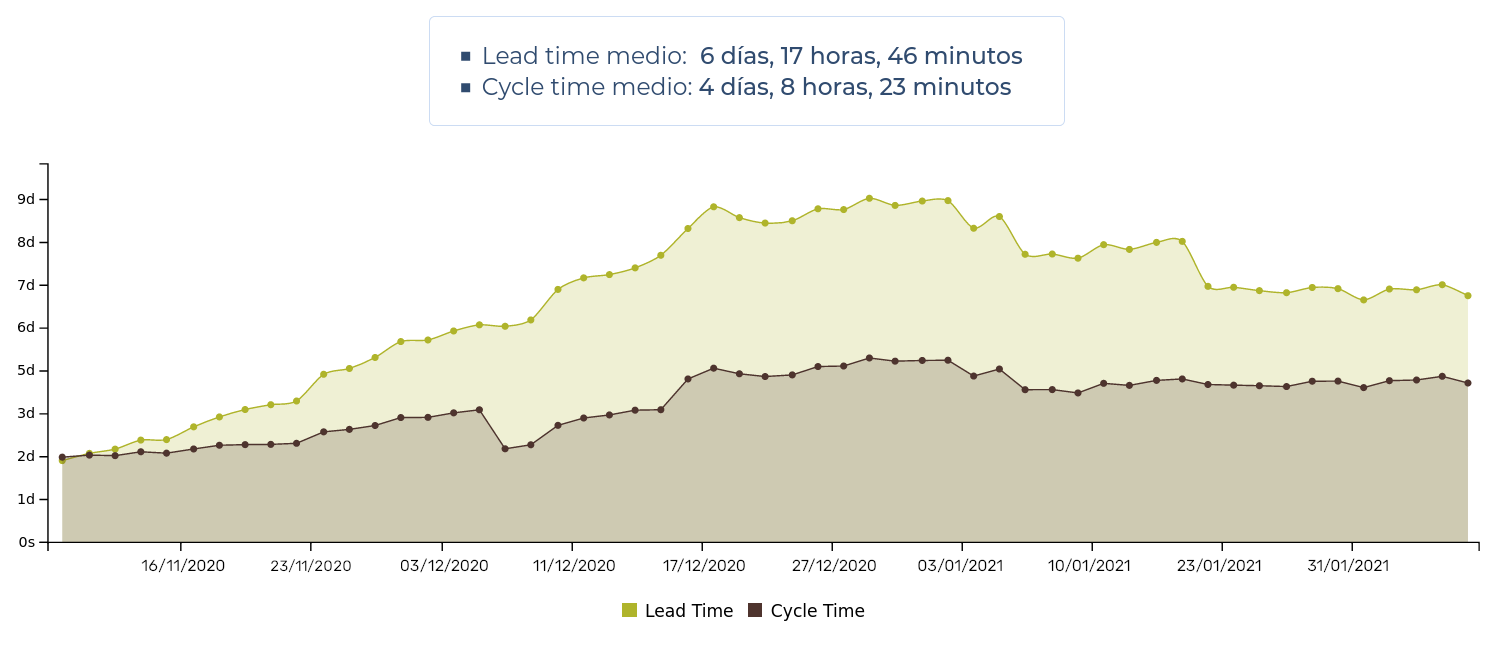
\includegraphics[width=\textwidth]{average-lead-cycle}
	\vspace{-0.7cm}
	\caption{Gráfico de \emph{lead} y \emph{cycle time} medios.}
	\label{average-lead-cycle}
\end{figure}

Como vemos en la \hyperref[average-lead-cycle]{anterior figura}, el \emph{lead time} medio fue de algo menos de 7 días, y el \emph{cycle time} de 4 días y 8 horas. Como es lógico, las primeras tareas se completaron más rápido, pero según la complejidad de las mismas fue incrementándose, también se reflejo en los tiempos. En el punto central del proyecto, se alcanzó una media de \emph{lead time} de 9 días, aunque el \emph{cycle time} se mantuvo por debajo de los 5, lo que indica que existía un mayor número de tareas esperando a ser atendidas.

Otro de los gráficos propios de Kanban que nos puede ofrecer información valiosa es el llamado diagrama de flujo acumulado (CFD, por sus siglas en inglés). Este gráfico muestra el número de tareas que hay en cada columna a lo largo del tiempo.

\begin{figure}[h]
	\centering
	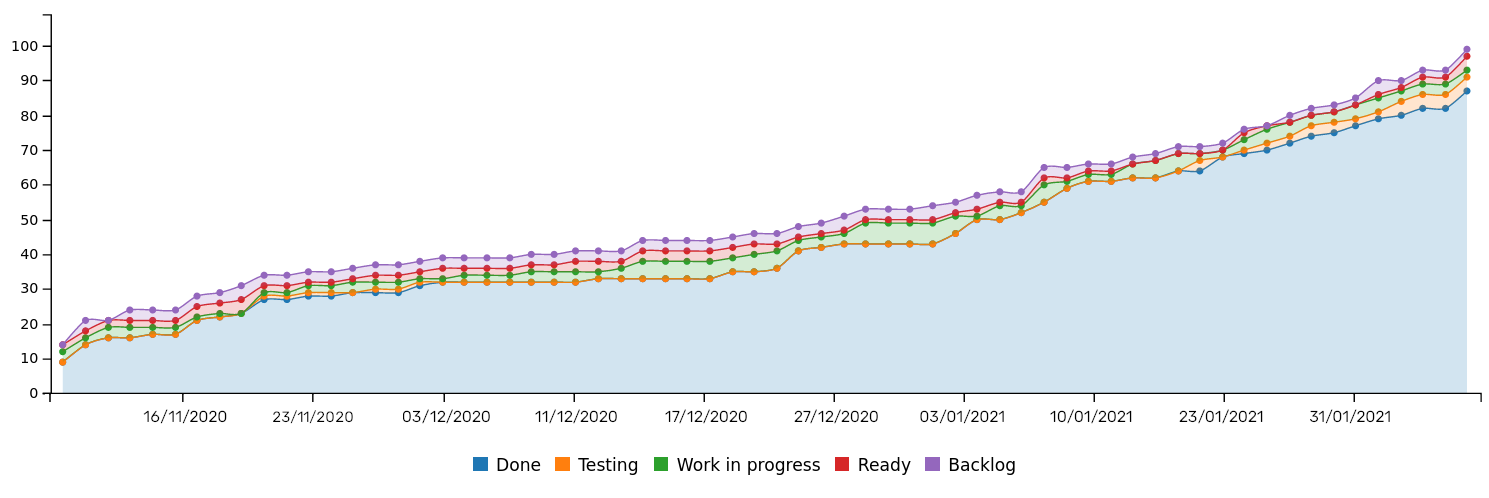
\includegraphics[width=\textwidth]{cfd}
	\vspace{-0.7cm}
	\caption{Diagrama de flujo acumulado desde el comienzo del proyecto.}
	\label{cfd}
\end{figure}

Como podemos ver en el \hyperref[cfd]{anterior diagrama}, el trabajo en las diferentes columnas se distribuyó de forma correcta, no apareciendo grandes diferencias entre ellas. En este gráfico, también podemos apreciar que en la parte central del proyecto, las tareas en <<\emph{Work in progress}>> fueron algo mayores que en el resto de columnas, lo cual es comprensible.

El diagrama de flujo acumulado obtenido muestra también que el ritmo de trabajo fue constante, incrementándose ligeramente hacia el final del proyecto.

Podemos visualizar también la distribución de las tareas en función de su tipo:

\begin{figure}[h]
	\centering
	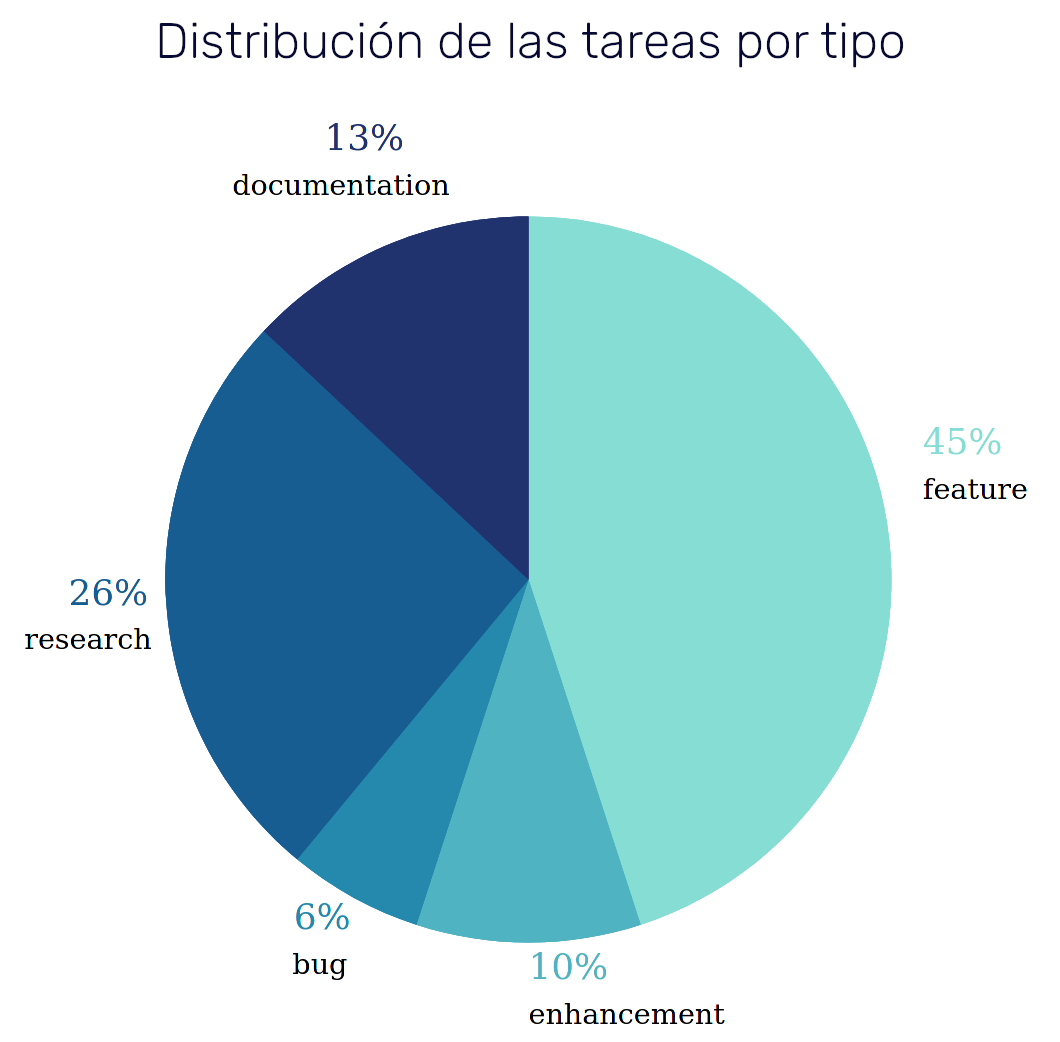
\includegraphics[width=0.7\textwidth]{distribucion-tareas}
	\caption{Distribución de las tareas según su tipo.}
\end{figure}

Como es lógico, la mayor parte de las tareas se dedicaron a ofrecer nuevas funcionalidades (\emph{feature}), aunque gran número de ellas se dedicaron al aprendizaje y búsqueda de información (\emph{research}), lo cual también parece ajustarse a la realidad, puesto que como ya hemos mencionado, muchas de las herramientas y técnicas que hemos utilizado eran nuevas para nosotros. 

Para finalizar esta sección, cabe mencionar que en el \href{https://github.com/dmlls/jizt/milestones}{repositorio del proyecto}, y en su \href{https://board.jizt.it/public/board/c08ea3322e2876652a0581e79d6430e2dc0c27720d8a06d7853e84c3cd2b}{tablero Kanban}, se puede encontrar información más detallada de cada historia de usuario y \emph{epic}.

\newpage

\section{Estudio de viabilidad}

\subsection{Viabilidad económica}

Uno de los puntos cruciales a la hora de estudiar la viabilidad de un proyecto, y que en muchos casos determina el éxito o el fracaso del mismo, es la viabilidad económica.

En esta sección analizamos los costes y beneficios de JIZT.


\subsubsection{Costes del proyecto}

En nuestro caso, dividiremos los costes del proyecto n costes fijos, directos e indirectos.

\vspace{0.4cm}
\noindent
\textbf{\emph{Costes fijos}}

Los costes fijos son aquellos costes invariables que debemos abonar, independientemente del desarrollo del proyecto \cite{perez18}.

\begin{table}[h!]
	\centering
	\begin{tabular}{>{\raggedright}b{0.6\linewidth}>{\raggedleft\arraybackslash}b{0.2\linewidth}}
		\toprule
		\textbf{{\scriptsize CONCEPTO}}  & \textbf{{\scriptsize IMPORTE}} \\
		\midrule
		\small{\; Servicio de Internet} & \small{200,00 €} \\
		\midrule
		\small{\; Servicio de Luz$^1$} & \small{225,00 €} \\
		\midrule
		\small{\; Materiales de oficina} & \small{5,00 €} \\
		\midrule
		\small{\; Salarios$^2$} & \small{9911,88 €} \\
		\scriptsize{\qquad Salario mensual neto} & \scriptsize{1000,00 €} \\
		\scriptsize{\qquad Retenciones1 por IRPF (24 \%)$^3$} & \scriptsize{528,63 €} \\
		\scriptsize{\qquad Cuotas a la Seg. Social (30,6 \%)$^4$} & \scriptsize{674,01 €} \\
		\scriptsize{\qquad Salario mensual bruto} & \scriptsize{2202,64 €} \\
		\bottomrule
		\textbf{{\scriptsize TOTAL}}  & \textbf{\small 10341,88 €} \\
		\bottomrule
		\multicolumn{2}{l}{\scriptsize{$^1$ Costes calculados para 4,5 meses, con tarifa de mercado libre y potencia}} \\
		\multicolumn{2}{l}{\hspace{0.11cm} \scriptsize{contratada de 3,3 kW (precio mensual medio de 50 €).}} \\
		\multicolumn{2}{l}{\scriptsize{$^2$ Costes calculados para 4,5 meses.}} \\
		\multicolumn{2}{l}{\scriptsize{$^3$ Según la tabla de retenciones por IRPF aplicable al ejercicio 2021 \cite{irpf21}}} \\
		\multicolumn{2}{l}{\scriptsize{$^4$ Porcentaje para autónomos según la Ley 11/2020, de 30 de diciembre, de}} \\
		\multicolumn{2}{l}{\hspace{0.11cm} \scriptsize{Presupuestos Generales del Estado para el año 2021 \cite{boe341}.}} \\
		\bottomrule
	\end{tabular}
	\caption{Desglose de costes fijos del proyecto.}
\end{table}

\newpage

\noindent
\textbf{\emph{Costes directos}}

Los costes directos son aquellos costes derivados directamente del desarrollo del proyecto.

\begin{table}[h!]
	\centering
	\begin{tabular}{>{\raggedright}m{0.58\linewidth}>{\raggedleft}m{0.16\linewidth}>{\raggedleft\arraybackslash}m{0.15\linewidth}}
		\toprule
		\textbf{{\scriptsize CONCEPTO}}  & \textbf{{\scriptsize IMPORTE}} & \textbf{{\scriptsize IMPORTE AMORTIZ.}} \\
		\midrule
		\small{\; Costes de \emph{hardware}$^1$} & \small{2509,58 €} & \small{79,49 €} \\
		\scriptsize{\qquad Ordenador personal} & \scriptsize{845,00 €} & \scriptsize{63,37 €} \\
		\scriptsize{\qquad \emph{Smartphone} Android} & \scriptsize{215,00 €} & \scriptsize{16,12 €} \\
		\scriptsize{\qquad Servicio GKE$^2$ de Google Cloud} & \scriptsize{1449,58 €} & - \\
		\midrule
		\small{\; Costes de \emph{software}$^3$} & \small{89,95 €} & \small{16,86 €} \\
		\scriptsize{\qquad Adobe Illustrator} & \scriptsize{89,95 €} &  \scriptsize{16,86 €} \\

	
		\bottomrule
		\textbf{{\scriptsize TOTAL}}  & \textbf{\small 2599,53 €} & \textbf{\small 96,35 €} \\
		\bottomrule
		\multicolumn{3}{l}{\scriptsize{$^1$ Se han calculado con una amortización de 5 años, habiendo sido utilizado 4,5 meses.}} \\
		\multicolumn{3}{l}{\scriptsize{$^2$ Google Kubernetes Engine \cite{gke}.}} \\
		\multicolumn{3}{l}{\scriptsize{$^1$ Se han calculado con una amortización de 2 años, habiendo sido utilizado 4,5 meses.}} \\
		\bottomrule
	\end{tabular}
	\caption{Desglose de costes directos del proyecto.}
\end{table}

\noindent
\textbf{\emph{Costes indirectos}}

Los costes indirectos son aquellos que no dependen directamente del desarrollo del proyecto.

\begin{table}[h!]
	\centering
	\begin{tabular}{>{\raggedright}b{0.6\linewidth}>{\raggedleft\arraybackslash}b{0.2\linewidth}}
		\toprule
		\textbf{{\scriptsize CONCEPTO}}  & \textbf{{\scriptsize IMPORTE}} \\
		\midrule
		\small{\; Dominio \href{https://www.jizt.it}{jizt.it}} & \small{4,81 €} \\
		\small{\; Cuenta de Google Play} & \small{20,76 €} \\
		\small{\; Impresión de la Memoria y el cartel del TFG} & \small{40,00 €} \\
		\bottomrule
		\textbf{{\scriptsize TOTAL}}  & \textbf{\small 65,57 €} \\
		\bottomrule
	\end{tabular}
	\caption{Desglose de costes indirectos del proyecto.}
\end{table}

\noindent
\textbf{\emph{Costes totales del proyecto}}

Considerando las tres categorías de costes recogidas anteriormente, la suma de los costes totales del proyecto asciende a \textbf{13006,10 €}.

\newpage

\subsubsection{Beneficios}

La API REST de JIZT se ofrece en tres planes de suscripción diferentes.

\vspace{-0.3cm}
\begin{itemize}[\textbullet]
	\item \textbf{\emph{Gratuito}}: este plan se ajusta a las necesidades de cualquier usuario regular que no vaya a realizar un uso exhaustivo del servicio. Se permiten 5.000 peticiones a la API REST, pudiendo hacerse hasta 5 peticiones por minuto. No incluye soporte técnico.
	
	\item \textbf{Estándar}: para aquellas empresas o particulares que van a realizar un uso más intensivo del servicio. Se incluyen 15.000 peticiones a la API REST, pudiendo hacerse hasta 15 peticiones por minuto. Incluye soporte técnico y de integración. El precio es de 166 €/mes.
	
	\item \textbf{Personalizado}: para aquellos usuarios cuyas necesidades no encajen en ninguno de los anteriores precios. El precio se establecerá en función de los requerimientos concretos del usuario.
\end{itemize}

En cuanto a la aplicación, es totalmente gratuita y no contiene publicidad.

\newpage
\subsection{Análisis DAFO}

Tras llevar a cabo un pequeño análisis de mercado, hemos identificado que las principales debilidades, amenazas, fortalezas y oportunidades de nuestro proyecto son las siguientes:

\begin{figure}[h]
	\centering
	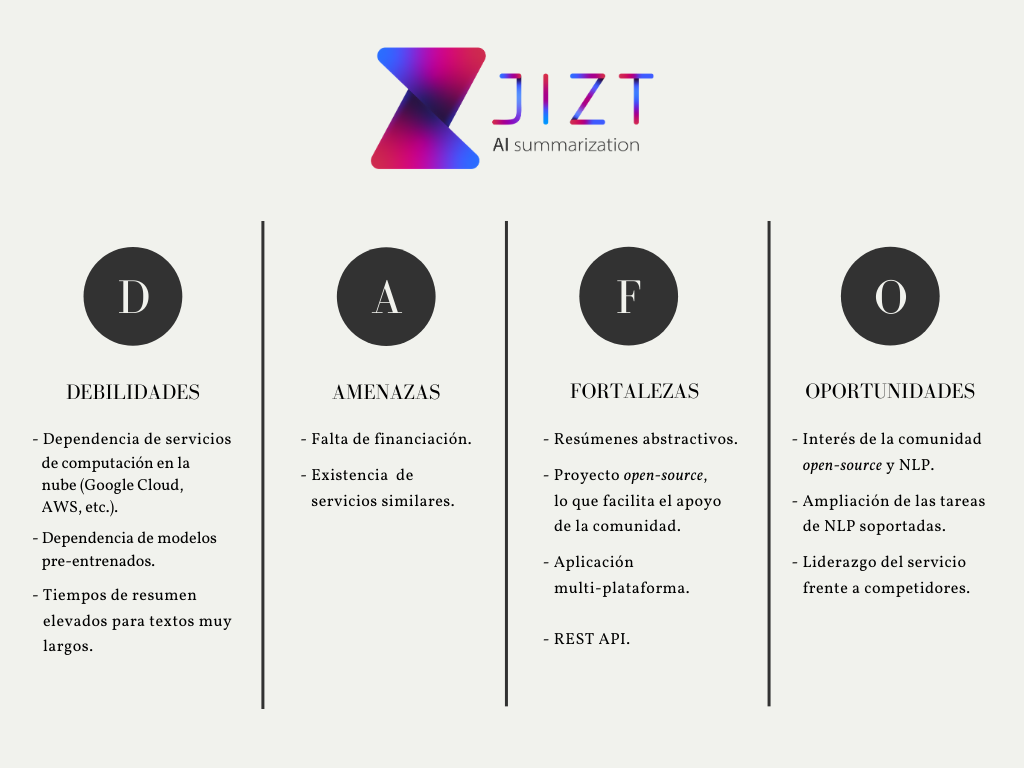
\includegraphics[width=1\textwidth]{dafo}
	\vspace{-0.5cm}
	\caption{Análisis DAFO de JIZT.}
\end{figure}

\subsection{Viabilidad legal}

\subsubsection{Licencia del código fuente del proyecto}

Desde un primer momento nuestra intencción era licenciar el proyecto bajo una licencia de \emph{Software} Libre. Dentro de este entorno, se han considerado las tres licencias más extendidas: Apache-2.0, MIT, y GPLv3.

Tras una lectura exhaustiva de las cláusulas de cada una de ellas, así como de opiniones en \emph{blogs}, charlas, foros, etc., y tras una profunda reflexión, considerando especialmente la licencia MIT y la GPLv3, hemos tomado la decisión de que nuestro software estará licenciado bajo \textbf{GNU GPLv3} \cite{gplv3}, cuyos puntos principales se recogen en la \autoref{gnu-gpl3}.

\begin{figure}[h]
	\centering
	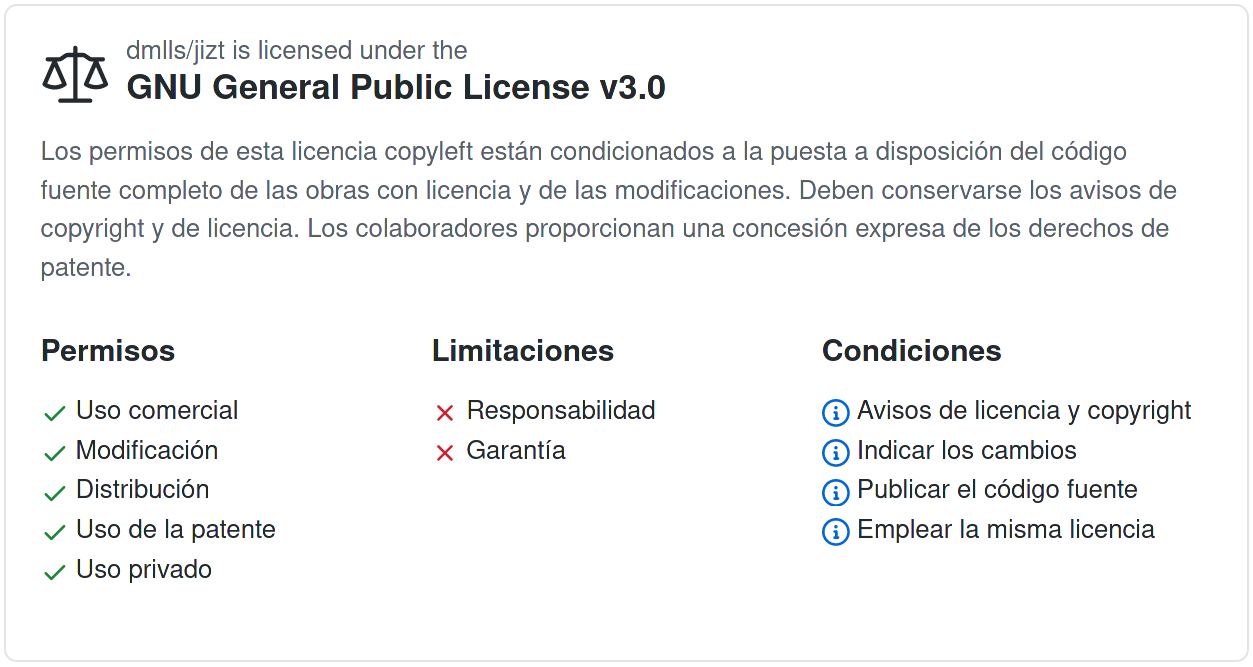
\includegraphics[width=1\textwidth]{gnu-gpl3}
	\vspace{-0.5cm}
	\caption[Resumen de la licencia GNU GPLv3]{Resumen de la licencia GNU GPLv3. Imagen extraída y traducida de \href{https://github.com/dmlls/jizt/blob/main/LICENSE}{https://github.com/dmlls/jizt/blob/main/LICENSE}.}
	\label{gnu-gpl3}
\end{figure}

Se puede acceder a la licencia completa a través de \href{https://www.gnu.org/licenses/gpl-3.0.en.html}{https://www.gnu.org/\newline licenses/gpl-3.0.en.html}.

Las principales razones de nuestra elección son:

\vspace{-0.3cm}
\begin{itemize}[\textbullet]
	\item Pese a que la licencia MIT pueda parecer más permisiva en un primer lugar, ya que no obliga a que el código fuente se mantenga abierto en un futuro, creemos que a largo plazo esta <<permisividad>>, paradójicamente, puede resultar en una limitación de sí misma. Esto es, el hecho de que ese supuesto \emph{software} <<libre>> se pueda volver \emph{software} <<cerrado>>, lo excluye en primer lugar de esa definición de <<libre>>, en nuestra opinión.

	\item Este proyecto no podría existir sin las contribuciones de \emph{software} libre anteriores. Por ello, queremos asegurar que este proyecto siempre se mantenga abierto para poder ayudar a otros y retroalimentarse con los aportes de la comunidad.
	
	\item El simple hecho de elegir una licencia, conlleva un sinnúmero de implicaciones morales, económicas, sociales, etc., pero es algo necesario, ya que el \emph{software} sin licencia explícita se toma por defecto como \emph{copyright}.
\end{itemize}

\newpage

\noindent
\textbf{Listado de dependencias}

Todas las dependencias del proyecto se encuentran licenciadas bajo licencias compatibles con GNU GPLv3.

A continuación, se recoge una lista detallada de las mismas:

\begin{table}[h!]
	\centering
	\begin{tabular}{>{\raggedright}b{0.28\linewidth}>{\raggedright}b{0.15\linewidth}>{\raggedright}b{0.3\linewidth}>{\raggedleft\arraybackslash}b{0.15\linewidth}}
		\toprule
		\textbf{Dependencia} & \textbf{Versión} & \textbf{Descripción} & \textbf{Licencia} \\
		\midrule
		\small{\; API REST} & & & \\
		\small{\qquad \texttt{NLTK}} & \small{3.5} & \scriptsize{Utilidades de NLP.} & \small{Apache v2.0} \\
		\small{\qquad \texttt{transformers}} & \small{4.1.1} & \scriptsize{Modelos pre-entrenados.} & \small{Apache v2.0} \\
		\small{\qquad \texttt{truecase}} & \small{0.0.12} & \scriptsize{\emph{Truecaser}.} & \small{Apache v2.0} \\
		\small{\qquad \texttt{confluent}-} & \small{1.5.0} & \scriptsize{Cliente de Kafka para} & \small{Apache v2.0}  \\
		\small{\qquad \texttt{kafka}} & & \scriptsize{Python.} & \\
		\small{\qquad \texttt{strimzi}-} & \small{0.21.0} & \scriptsize{Kafka en Kubernetes.} & \small{Apache v2.0}  \\
		\small{\qquad \texttt{operator}} & & & \\
		\small{\qquad \texttt{postgres}-} & \small{4.5.1} & \scriptsize{PostgreSQL en Kubernetes.} & \small{Apache v2.0}  \\
		\small{\qquad \texttt{operator}} & & & \\
		\small{\qquad \texttt{blingfire}} & \small{0.1.3} & \scriptsize{Utilidades de NLP.} & \small{MIT} \\
		\small{\qquad \texttt{marshmallow}} & \small{4.5.1} & \scriptsize{Serialización y de-} & \small{Apache v2.0}  \\
		& & \scriptsize{serialización.} & \\
		
		\midrule
		
		\small{\; Aplicación} & & & \\
		\small{\qquad \texttt{hive}} & \small{1.4.4+1} & \scriptsize{Base de datos noSQL.} & \small{Apache v2.0} \\
		\small{\qquad \texttt{flutter\_bloc}} & \small{6.1.2 } & \scriptsize{Patrón bloc en Flutter.} & \small{MIT} \\
		\small{\qquad \texttt{flutter\_svg}} & \small{0.19.2+1} & \scriptsize{Soporte para SVG.} & \small{MIT} \\
		\small{\qquad \texttt{clipboard}} & \small{0.1.2+8} & \scriptsize{Portapapeles.} & \small{BSD} \\
		\small{\qquad \texttt{json\_}} & \small{3.5.1} & \scriptsize{Serialización de JSON.} & \small{BSD} \\
		\small{\qquad \texttt{serializable}} & & & \\
		\small{\qquad \texttt{json\_}} & \small{3.1.1} & \scriptsize{Anotaciones de JSON.} & \small{BSD} \\
		\small{\qquad \texttt{annotation}} & & & \\
		\small{\qquad \texttt{share}} & \small{0.6.5+4} & \scriptsize{Soporte para compartir en} & \small{BSD} \\
		& & \scriptsize{diferentes plataformas.} & \\
		\small{\qquad \texttt{http}} & \small{0.12.2} & \scriptsize{Soporte para HTTP.} & \small{BSD} \\
		\bottomrule
	\end{tabular}
	\caption{Listado de dependencias.}
\end{table}1

\subsubsection{Licencia de la documentación del proyecto}

La totalidad de la documentación de JIZT se distribuye bajo licencia GNU Free Documentation License (GFDL) \cite{gfdl}.

Esta licencia es una adaptación al contexto de la documentación de la GNU General Public License (GPL), la cual está pensada para licenciar código fuente.

La GFDL da permiso a los lectores de copiar, redistribuir y  modificar una obra (excepto las <<secciones invariables>>) y exige que todas las copias y derivados estén disponibles bajo la misma licencia. Las copias también pueden venderse comercialmente, pero, si se producen en grandes cantidades (más de 100), el documento original o el código fuente deben ponerse a disposición del destinatario de la obra \cite{gfdl}.

Se puede acceder a la licencia completa en \href{https://www.gnu.org/licenses/fdl-1.3.html}{https://www.gnu.org/licenses/\newline fdl-1.3.html}.


\subsubsection{Licencia de la Memoria y los Anexos del proyecto}

Los documentos referentes a la Memoria y a los Anexos (excepto los apéndices  \hyperref[apendice:programador]{D:  Documentación técnica de programación} y \hyperref[apendice:usuario]{E: Documentación de usuario}), se encuentran licenciados bajo Creative Commons Atribución-CompartirIgual 4.0 Internacional (CC BY-SA 4.0).

Esta licencia se puede resumir en los siguientes puntos \cite{creative-commons}:

\vspace{-0.2cm}
\begin{itemize} [\textbullet]
	\item Cualquiera es libre de:
	\begin{itemize} [◦]
		\item Compartir: copiar y redistribuir el material en cualquier medio o formato.
		
		\item  Adaptar: remezclar, transformar y construir a partir del material para cualquier propósito, incluso comercialmente. 
	\end{itemize}
	\item Bajo los siguientes términos:
	\begin{itemize} [◦]
		\item Atribución: se debe dar crédito de manera adecuada, brindar un enlace a la licencia, e indicar si se han realizado cambios. Puede hacerse en cualquier forma razonable, pero no de forma tal que sugiera que aquel que lo usa, o su uso tienen el apoyo del licenciante.
		
		\item \emph{CompartirIgual}: si remezcla, transforma o crea a partir del material, debe distribuir su contribución bajo la la misma licencia del original.
	\end{itemize}
\end{itemize}

Se puede acceder a la licencia completa a través de \\ \href{https://creativecommons.org/licenses/by-sa/4.0/legalcode.es}{https://creativecommons.org/licenses/by-sa/4.0/legalcode.es}.